\documentclass{article}
% \usepackage[margin=1in]{geometry}
\usepackage{amsmath, amssymb, amsthm}
\usepackage{parskip}
\usepackage{tikz}
\usepackage{enumerate}
\usepackage[T1]{fontenc}

%%%%%%%%% Useful shorthand %%%%%%%%%%%%
\newcommand{\0}{\underline{0}}
\newcommand{\1}{\underline{1}}
\newcommand{\2}{\underline{2}}
\newcommand{\N}{\mathbb{N}}
\renewcommand{\S}{\mathcal{S}}
%%%%%%%%%%%%%%%%%%%%%%%%%%%%%%%%%%%%%%%

\title{Notes on Transducer Orbit Checking}
\author{Evan Bergeron}
\begin{document}
\maketitle

\subsection*{A Simple Invertible Transducer}
This is $A^3_2$.
\begin{center}
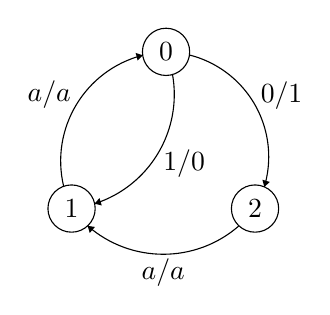
\begin{tikzpicture}[scale=0.1]
\tikzstyle{every node}+=[inner sep=0pt]
\draw [black] (39.5,-18.5) circle (3);
\draw (39.5,-18.5) node {$0$};
\draw [black] (50.8,-38.4) circle (3);
\draw (50.8,-38.4) node {$2$};
\draw [black] (27.5,-38.4) circle (3);
\draw (27.5,-38.4) node {$1$};
\draw [black] (40.322,-21.38) arc (10.02185:-72.20308:14.565);
\fill [black] (30.43,-37.78) -- (31.34,-38.01) -- (31.04,-37.06);
\draw (39.09,-32.7) node [right] {$1/0$};
\draw [black] (42.467,-18.9) arc (75.86616:-16.68694:13.324);
\fill [black] (51.98,-35.65) -- (52.68,-35.02) -- (51.73,-34.74);
\draw (51.46,-24.02) node [right] {$0/1$};
\draw [black] (48.761,-40.593) arc (-48.81225:-131.18775:14.594);
\fill [black] (29.54,-40.59) -- (29.81,-41.5) -- (30.47,-40.74);
\draw (39.15,-44.7) node [below] {$a/a$};
\draw [black] (26.496,-35.579) arc (-166.604:-255.57722:13.874);
\fill [black] (36.54,-18.93) -- (35.64,-18.64) -- (35.89,-19.61);
\draw (27.47,-23.93) node [left] {$a/a$};
\end{tikzpicture}
\end{center}
Let $\underline{i}$ be the function induced by applying $A^3_2$ to some string with state $i$ as the start state. $\0, \1, \2$ generate a semigroup under composition. For example, $\0^2$ is the result of applying $\0$ twice. We call such functions \textit{transductions}.

If $x$ is some string, call $\0^* = \{ \0^t(x) \mid t \in \N \}$ the \textit{orbit} of $x$ under $\0$.

We prove that checking if $y \in \0^*(x)$ is in P. We then investigate orbit checking for arbitrary $f$ in the semigroup.

\subsection*{A Necassary Condition}
Let $f = \0$. Let $y \in f^*(x)$. Let $c$ be a sequence where $c_i$ is the number of times $x_i$ is flipped on the way to $y$. Then we claim that
\begin{align*}
c_i &= \lfloor (c_{i-3} / 2) \rfloor + (c_{i-3} \mod{2}) \cdot (1 - x_{i-3})\\
    &+\lfloor (c_{i-2} / 2) \rfloor + (c_{i-2} \mod{2}) \cdot x_{i-2}
\end{align*}
where $c_0$ is the index of $y$ in $f^*(x)$, $c_1$ is 0, and $c_2$ is $\lfloor c_0 / 2 \rfloor$.

$x_0$ is flipped upon every invocation of $f$. $x_1$ is never flipped. $x_2$ is flipped roughly every other time $x_0$ is flipped. That is, it's flipped every time $x_0$ changes from a 1 to a 0. Without loss, we may assume $x_0 = 0$. Thus, $c_2 = \lfloor c_0 / 2 \rfloor$ (it's not flipped the first time, but then is flipped every other time afterward).

Consider some application of $f$. $c_i$ is flipped iff $c_{i-2}$ is flipped from a 1 to a 0 or $c_{i-3}$ is flipped from a 0 to a 1. If $c_{i-2}$ and $c_{i-3}$ are even, then this is precisely every other flip. If either $c_{i-2}$ or $c_{i-3}$ is odd, then $c_i$ is dependent on both $c_{i-2}$ and $c_{i-3}$ as well as the initial conditions in $x$. We add one depending on whether or not the first flip of $c_{i-2}$, $c_{i-3}$ causes $c_i$ to flip as well.

\subsection*{A Sufficient Condition}
Let $p$ be a sequence where $p_i = c_i \mod{2}$ for all $i$. Then if $x \oplus y$ looks like some $p$, then $y \in f^*(x)$. That is, if you fix your initial conditions and the above recurrence holds through $x \oplus y$, then $y \in f^*(x)$.

That being said, we necassarily don't know $c_0$.

\subsection*{$A^3_2$ Orbit Checking is in NP}
Our verifier takes in two strings $x$, $y$, and an index $i$. This index is the position of $y$ in $x$'s orbit. WLOG, suppose $x_0 = 1$. We first set $c_0 = i$, $c_1 = 0$, and $c_2 = \lfloor c_0 / 2 \rfloor$. We then calculate $c_i$ and check that $c_i \mod 2 = x_i \oplus y_i$ for all $i$.

The certificate is poly length with respect to $x$ and $y$, as the orbit of $y$ has length at most $2^n$ (so the length of an index is at most $n$).


% \subsection*{A Rephrasing of the Problem}
% In orbit iff there is a $t$ such that $y = f^t(x)$. Suffices to find this $t$.

\subsection*{Derivatives}
We introduce the notion of so-called derivatives. They're named as such because they resemble normal calculus derivatives in many ways, though that's currently beyond my knowledge.

If $f_u$ is the transduction corresponding to some state state $u$ of a transducer, then $\partial_b(f_u) = f_v$ if state $u$ transitions to state $v$ on input $b$. Each transducer has a corresponding derivative table, which is effectively an adjacency list representation of the transducer.

For example, $A^3_2$ has the following representation:

\begin{itemize}
\item $\partial_0(\0) = \2$
\item $\partial_1(\0) = \1$
\item $\partial_b(\2) = \1$ for any $b$
\item $\partial_b(\1) = \0$ for any $b$
\end{itemize}

\subsection*{Semigroups Revisited}
Recall that the states of $A^3_2$ form a semigroup $\S(A^3_2)$. This semigroup is commutative - it doesn't matter what order we apply the transductions in. This follows by commutativity of addition modulo 2 (suffices to consider each bit one at a time). This means that every element in $\S(A^3_2)$ looks like $\0^i \1^j\2^k$ for $i, j, k \in \N$.

Further, we have an identity element in $\S(A^3_2)$: $$\0^2\1^2\2 = I$$
\begin{proof}
% TODO - not sure how this one works. It suffices to show that $c_i$ is even for all $i$.
Proof by induction - it suffices to show that $c_i$ is even for all $i$. In fact, $c_i$ will be 2.

$c_0$ is 2, each of the applications of $\0$ flip $x_0$ once. The applications of $\1$ and $\2$ skip it. $c_1$ is also 2 as each application of $\1$ flips $x_1$ once and $\0$ and $\2$ skip it. $c_2 = 2$ - $\2$ flips it once, $\1^2$ skips it, and exactly one of the two applications of $\0$ flip it.

Then $c_{i-2} = c_{i-3} = 2$ by induction, so
\begin{align*}
c_i &= \lfloor (c_{i-3} / 2) \rfloor + \lfloor (c_{i-2} / 2) \rfloor = 1 + 1 = 2
\end{align*}
\end{proof}
This means that $\S(A^3_2)$ is already a group ($\0^{-1} = \0\1^2\2$ and so on).

\subsection*{The $A^3_2$ Orbit Relation is Rational}
This is hard - need to write that vector reduction thing.

\subsection*{A New Class of Transducers - 1-Toggle-1-Split}

\subsection*{1-Tog-1-Split Orbit Checking in P?}

\subsection*{1-Tog-1-Split Orbit Relation Rational?}

\subsection*{1-Tog Orbit Relation Rational?}

TODO: Automate making the orbit automaton?

\end{document}
